% arara: xelatex
% arara: biber
% arara: xelatex
% arara: xelatex
%%% arara: clean: { files: [riemann_main.log,riemann_main.aux,riemann_main.blg,riemann_main.bbl,riemann_main.bcf,riemann_main.toc,riemann_main.run.xml] }
%%% arara: lmkclean
%%% arara: pdflatex
%%% arara: pdflatex
%%% % arara: lmkclean
%%% zsh> setopt no_nomatch

% Chandra Images by Category: Supernovas & Supernova Remnants
% https://chandra.harvard.edu/photo/category/snr.html

\documentclass[a4paper,12pt]{extarticle}

\RequirePackage[l2tabu,orthodox]{nag} % Раскомментировав, можно в логе получать рекомендации относительно правильного использования пакетов и предупреждения об устаревших и нерекомендуемых пакетах
% \documentclass[a4paper,14pt]{extarticle}
\usepackage[left=1.5 cm,right=1.6cm,top=1.5cm,bottom=2.5cm]{geometry}

%%% Mathematical packages %%%
\usepackage{amsthm,amsmath,amscd} % Математические дополнения от AMS
\usepackage{amsfonts,amssymb}     % Математические дополнения от AMS
\usepackage{mathtools}            % Добавляет окружение multlined
\usepackage{mathtext}
\usepackage{cancel}

\usepackage{textcomp}

\RequirePackage{ifxetex, ifluatex}
\ifxetex
  % https://tex.stackexchange.com/a/38631
  \renewcommand{\mathbf}{\ensuremath{\symbf}}
  \usepackage{unicode-math}
  \usepackage{polyglossia}                        % Поддержка многоязычности (fontspec подгружается автоматически)
 % \setmainlanguage[babelshorthands=true]{russian} % Язык по-умолчанию русский с поддержкой приятных команд пакета babel
  \setotherlanguage{english}                      % Дополнительный язык = английский (в американской вариации по-умолчанию)
  % Семейство шрифтов Liberation (https://pagure.io/liberation-fonts)
  \setmonofont{LiberationMono}[Scale=0.87]        % моноширинный шрифт
  \newfontfamily\cyrillicfonttt{LiberationMono}[  % моноширинный шрифт для кириллицы
    Scale=0.87]
  \defaultfontfeatures{Ligatures=TeX}             % стандартные лигатуры TeX, замены нескольких дефисов на тире и т. п. Настройки моноширинного шрифта должны идти до этой строки, чтобы при врезках кода программ в коде не применялись лигатуры и замены дефисов
  \setmainfont{LiberationSerif}                   % Шрифт с засечками
  \newfontfamily\cyrillicfont{LiberationSerif}    % Шрифт с засечками для кириллицы
  \setsansfont{LiberationSans}                    % Шрифт без засечек
  \newfontfamily\cyrillicfontsf{LiberationSans}   % Шрифт без засечек для кириллицы

  % fake small capitals
  % https://tex.stackexchange.com/questions/55664/fake-small-caps-with-xetex-fontspec
  \makeatletter
  \newlength\fake@f
  \newlength\fake@c
  \def\textsc#1{%
    \begingroup%
    \xdef\fake@name{\csname\curr@fontshape/\f@size\endcsname}%
    \fontsize{\fontdimen8\fake@name}{\baselineskip}\selectfont%
    \MakeUppercase{#1}%
    \endgroup%
    }
  \makeatother
  % \renewcommand{\textsc}[1]{\fauxschelper#1 \relax\relax}
  % \def\fauxschelper#1 #2\relax{%
  %   \fauxschelphelp#1\relax\relax%
  %   \if\relax#2\relax\else\ \fauxschelper#2\relax\fi%
  %   }
  % \def\Hscale{.83}\def\Vscale{.72}\def\Cscale{1.00}
  % \def\fauxschelphelp#1#2\relax{%
  %   \ifnum`#1>``\ifnum`#1<`\{\scalebox{\Hscale}[\Vscale]{\uppercase{#1}}\else%
  %   \scalebox{\Cscale}[1]{#1}\fi\else\scalebox{\Cscale}[1]{#1}\fi%
  %   \ifx\relax#2\relax\else\fauxschelphelp#2\relax\fi}

\else
  \usepackage[T2A]{fontenc}           % кодировка
  \usepackage[utf8]{inputenc}         % Кодировка utf8
  \usepackage[english,russian]{babel} % Языки: русский, английский
\fi

\usepackage[colorlinks=true,unicode=true]{hyperref}

%%% Other packages %%%
\usepackage{xspace} % пробелы после предопределённых команд
\usepackage{color}
\usepackage{enumitem}
\usepackage{cmap}
\usepackage{array}
\usepackage{braket}
\usepackage{epsfig}
\usepackage{epstopdf}
\usepackage{graphicx}
\usepackage{float}
\usepackage{caption}
\captionsetup{compatibility=false}
\usepackage{subcaption}
\usepackage{indentfirst}
\usepackage{hyphenat}
\usepackage[normalem]{ulem}
\usepackage{wrapfig}
\usepackage{pdfpages}

\graphicspath{{img/}} % Пути к изображениям

%%% Toc %%%
% \setcounter{tocdepth}{4}
% \setcounter{secnumdepth}{4}

%%% Title %%%
% \usepackage{titlesec}
% \titleformat{\section}
% {\normalfont\large\bfseries}{\thesection}{1em}{}

%%% Setup bibliography %%%

\usepackage{csquotes} % biblatex рекомендует его подключать. Пакет для оформления сложных блоков цитирования.
%%% Загрузка пакета с основными настройками %%%
\makeatletter
\usepackage[%
backend=biber,% движок
bibencoding=utf8,% кодировка bib файла
sorting=none,% настройка сортировки списка литературы
style=gost-numeric,% стиль цитирования и библиографии (по ГОСТ)
language=autobib,% получение языка из babel/polyglossia, default: autobib % если ставить autocite или auto, то цитаты в тексте с указанием страницы, получат указание страницы на языке оригинала
autolang=other,% многоязычная библиография
clearlang=true,% внутренний сброс поля language, если он совпадает с языком из babel/polyglossia
defernumbers=true,% нумерация проставляется после двух компиляций, зато позволяет выцеплять библиографию по ключевым словам и нумеровать не из большего списка
sortcites=true,% сортировать номера затекстовых ссылок при цитировании (если в квадратных скобках несколько ссылок, то отображаться будут отсортированно, а не абы как)
movenames=false, % опция разрешает или запрещает перемещение имён в область сведений об ответственности, если количество имён больше трёх.
% не менять местами заголовок и список авторов, если авторов больше четырех
minnames=3, % сокращение списка имён
maxnames=4, % сокращение списка имён
doi=true,% Показывать или нет ссылки на DOI
isbn=false,% Показывать или нет ISBN, ISSN, ISRN
url=false,
eprint=true,
backref=true
]{biblatex}[2016/09/17]
%]{biblatex}
%\ltx@iffilelater{biblatex-gost.def}{2017/05/03}%
{\toggletrue{bbx:gostbibliography}%
\renewcommand*{\revsdnamepunct}{\addcomma}}{}
\makeatother

\DefineBibliographyStrings{english}{docthesis = {dissertation}}
\DefineBibliographyStrings{russian}{docthesis = {диссертация}}

% Custom backref Text
%https://tex.stackexchange.com/questions/196015/custom-backref-text
\DefineBibliographyStrings{english}{
  backrefpage  = {Цит. на с.\adddot},
  backrefpages = {Цит. на с.\adddot},
}
\DefineBibliographyStrings{russian}{
  backrefpage  = {Цит. на с.\adddot},
  backrefpages = {Цит. на с.\adddot},
}
\ifxetex
\else
% Исправление случая неподдержки знака номера в pdflatex
    \DefineBibliographyStrings{russian}{number={\textnumero}}
\fi

% разделитель ; для ссылок
\DeclareMultiCiteCommand{\multicites}[\mkbibbrackets]{\cite}{\addsemicolon\space}

%%% Colors %%%
\usepackage[dvipsnames]{xcolor}

\definecolor{linkcolor}{rgb}{0.08, 0.38, 0.74}
\definecolor{citecolor}{rgb}{0.18, 0.55, 0.34}
\definecolor{urlcolor}{rgb}{0.03, 0.57, 0.82}

\hypersetup{
    linktocpage=true,           % ссылки с номера страницы в оглавлении, списке таблиц и списке рисунков
    colorlinks,                 % ссылки отображаются раскрашенным текстом, а не раскрашенным прямоугольником, вокруг текста
    linkcolor={linkcolor},      % цвет ссылок типа ref, eqref и подобных
    citecolor={citecolor},      % цвет ссылок-цитат
    urlcolor={urlcolor},        % цвет гиперссылок
}

%%% Users commands %%%

\def\stella{\code{STEL\-LA}\xspace}
\def\millimetron{\code{Миллиметрон}\xspace}
\def\mesa{\code{ME\-SA}\xspace}
\def\supremna{\code{SUP\-REM\-NA}\xspace}

\def\araa{Annual Review of Astronomy and Astrophysics}
\def\apj{The Astrophysical Journal}
\def\apjl{The Astrophysical Journal Letters}
\def\apjs{The Astrophysical Journal Supplement}
\def\apss{Astrophysics and Space Science}
\def\azh{Астрон. Журнал}
\def\pazh{Письма в Астрон. Журнал}
\def\pasp{Pub. Astron. Soc. Pacific}
\def\pasa{Pub. Astron. Soc. Australia}
\def\prl{Phys. Rev. Lett}
\def\pre{Phys. Rev. E}
\def\sovast{Soviet Astronomy}
\def\aa{Astronomy and Astrophysics}
\def\aapr{Astronomy and Astrophysics Reviews}
\def\aj{Astronomical Journal}
\def\mnras{MNRAS}
\def\nat{Nature}
\def\ssr{Space Science Reviews}
\def\prd{Phys. Rev. D}
\def\jqsrt{Journal of Quantitative Spectroscopy and Radiative Transfer}

\DeclareRobustCommand{\todo}{\textcolor{red}}

\newcommand{\code}[1]{\texttt{#1}}
% \newcommand{\code}[1]{\textsc{#1}}
\newcommand\vecx[1]{\ifstrequal{#1}{0}{\ensuremath{\mathbf{0}}}{\ensuremath{\boldsymbol{#1}}}}

\newcommand\vecxu{\vecx{u}}



\newcommand{\pb}[1]{\textbf{\color{magenta}PB: #1}}
\newcommand{\iz}[1]{\textbf{\color{orange}IZ: #1}}

\newcommand\nifsx{$^{56}$Ni\xspace}
\newcommand\cofsx{$^{56}$Co\xspace}
\newcommand\fefsx{$^{56}$Fe\xspace}
\newcommand{\rsun}{\ensuremath{R_\odot}\xspace}
\newcommand{\msun}{\ensuremath{M_\odot}}

% 
\def\rej{\ensuremath{R_{\rm ej}}}
\def\mej{\ensuremath{M_{\rm ej}}}
\def\renv{\ensuremath{R_{\rm env}}}
\def\menv{\ensuremath{M_{\rm env}}}

\newcommand\snia{SN\,Ia\xspace}
\newcommand\snib{SN\,Ib\xspace}
\newcommand\snic{SN\,Ic\xspace}
\newcommand\sniib{SN\,IIb\xspace}
\newcommand\sniip{SN\,IIP\xspace}


\makeatletter
\@ifundefined{c@basement}{
  \newcounter{basement}
  \setcounter{basement}{0} % 0 --- hide basement;
                            % 1 --- show basement
}{}
\makeatother

\hyphenation{
  smooth-ed
  par-tic-le
  hy-dro-dy-nam-ics
}


%%% Add bibliography
\addbibresource{refs_hd_astro.bib}
\addbibresource{refs_hd_gydro.bib}

\begin{document}

%%% article title
\title{\large
 Заметки про космос, звезды, остатки сверхновых
}

\author{Илья~Заворохин, П.В.~Бакланов}

\date{\today}

\maketitle

\tableofcontents
\clearpage
%\newpage

%%%%% BEGIN
%------------------------------------------
%\section*{TODO}

%\begin{enumerate}

%\end{enumerate}

%------------------------------------------
\section{Введение}
\iz{Здесь я пытаюсь собирать данные относящиеся в основном к астрофизике и астрономии, поэтому гидрогазодинамики с задачей Римана в этом файле нет}
%------------------------------------------
\section{Историческая справка}
ауа
\iz{Имеет ли смысл писать что-то в таком разделе, что именно? стоит ли это вставлять в работу?}
%------------------------------------------
\section{Характерные масштабы процессов}
1 МэВ = $1.6\cdot 10^{-19} \hbox{Кл} \times 10^6 \hbox{В} = 1.6\cdot 10^{-13} \hbox{Дж}$
%------------------------------------------
\section{Физические понятия и законы}
\iz{Кажется в заметках имеет смысл перечислить основные законы. Пока здесь законы излучения тел}
\subsection{Закон смещения Вина}
Один из самых простых законов, которому подчиняется термодинамически равновесное излучение. 
Он гласит: длина волны, на которую приходится максимум спектральной плотность потока излучения абсолютно черного тела (АЧТ), обратно пропорциональна его абсолютной температуре и выражается формулой $$ \lambda_{max}=\frac{b}{T}$$ где $ b=0.0029$-постоянная Вина
\begin{figure}[!htb]
	\centering
	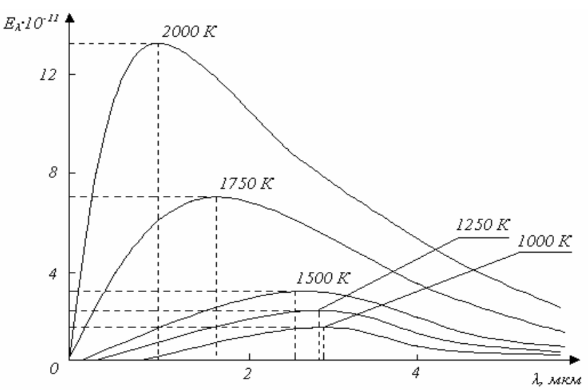
\includegraphics[width=0.6\textwidth]{Wien_displacement.png}
	\caption{
		График для пояснения закона смещения Вина
	}
	\label{fig:Wien_displacement}
\end{figure}
\subsection{Закон Рэлея-Джинса}
В классической физике плотность излучения абсолютно черного тела описывается законом Рэлея-Джинса:
$$\rho(\nu) \approx 8\pi\nu^2 kT/c^3,$$
где $\nu$ - частота излучения, k - постоянная Больцмана, T - абсолютная температура. В области низких частот формула Рэлея-Джинса хорошо описывает экспериментальные данные. Однако в области высоких частот расхождения с экспериментом были настолько существенны, что возникшую ситуацию стали называть «ультрафиолетовой катастрофой».
\subsection{Закон Стефана-Больцмана}
В 1879 году Йозеф Стефан на основе анализа экспериментальных данных пришёл к заключению, что интегральная светимость R(T) абсолютно черного тела пропорциональна четвертой степени абсолютной температуры Т:
$$R = \sigma T^4$$
Несколько позднее, в 1884 году Л.Больцман теоретически получил эту зависимость из термодинамических соображений. 
Числовое значение постоянной $\sigma = 5.671\cdot 10^{-8}$ Вт/$(\hbox{м}^2\cdot K^4)$
\\

\subsection{Закон Планка}
В 1900 г. была опубликована работа М. Планка, посвященная проблеме теплового излучения тел. Планк моделировал вещество как совокупность гармонических осцилляторов различной частоты $\nu$. Предположив, что излучение происходит не непрерывно, а порциями – квантами $h\nu$, он получил формулу распределения плотности энергии в спектре теплового излучения $\rho(T,\nu)$, которая хорошо согласовывалась с опытными данными
$$\rho(T,\nu)=\frac{8\pi h\nu^3}{c^3}\frac{1}{e^{h\omega/kT}-1}$$

\begin{figure}[!htb]
	\centering
	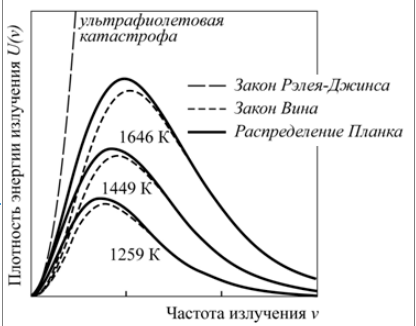
\includegraphics[width=0.4\textwidth]{energy_distribution_in_spectrum.png}
	\caption{
		Распределение энергии в спектре теплового излучения абсолютно черного тела.
	}
	\label{fig:energy_distribution_in_spectrum}
\end{figure}

\subsection{}
%------------------------------------------
\section{Остатки сверхновых}
\iz{Сейчас здесь перечислены типы сверхновых и стадии разлета остатка}

Сверхновая является заключительной стадией жизни некоторых звёзд.{\cite{Shklov1984}} В зависимости от внутреннего состава звезды вспышка может осуществляться разными механизмами и давать при этом разную картину на получаемых данных (кривых блеска). Выделяют 2 основных типа сверхновых: I и II. К I типу относят сверхновые, спектры которых не содержат линий водорода, ко II типу, наоборот, содержащие такие линии. Сверхновые I типа делят на 3 подтипа: Ia(есть кремний), Ib(есть гелий), Ic(нет гелия), а у II типа выделяют:1) по спектру IIb, IIn: 2)по кривой блеска(наличие плато) IIP и IIL. Сверхновые Ia существенно отличаются от всех остальных: считается что к нему приводит термоядерный взрыв, а ко всем остальным коллапс ядра массивной звезды.\\
\indent Сброшенная при вспышке сверхновой оболочка расширяется со сверхзвуковой скоростью в межзвездную среду и образует ударную волну. Различают несколько стадий взаимодействия оболочки с окружающей средой: свободный разлет, адиабатическое расширение, стадия снегоочистителя. Далее идет описание каждой стадии разлета.{\cite{Spitzer1981}}\\
\indentСтадия 1. Свободный разлет.\\
\indentНа этой стадии оболочка движется по инерции так, как если бы внешней среды не было вообще. $R(t)\propto t $ Излучение оболочки не играет роли в ее динамике. Стадия заканчивается при сгребании массы окружающего вещества, равной массе расширяющейся оболочки $M_0 = 4\pi/3\rho_0R^3$. Для $\rho_0=210^{-24}$ г/см$^3$ и $M_0=1M_{\theta}$ этот момент наступает при $R\approx 2$пк, примерно через 100 лет после начала расширения.\\
\indentСтадия 2. Адиабатическое расширение. \\
\indentРадиационные процессы по-прежнему динамически неважны (отсюда название - адиабатическая стадия), так как температура газа за фронтом ударной волны очень высокая. Кинетическая энергия оболочки расходуется на нагрев газа за фронтом сильной ударной волны и на ускорение сгребенного межзвездного газа. Когда масса сгребенного газа много больше $M_0$, движение оболочки довольно точно описывается автомодельным решением Л.И. Седова для сильного взрыва в среде. Можно получить зависимость поведения радиуса оболочки от времени из простых физических соображений. 
Пусть тепловая энергия газа, находящаяся в равновесии с кинетической, составляет долю $K_1$ от полной энергии $E$, а а давление непосредственно за фронтом УВ $p_2$ в $K_2$ раз больше среднего давления внутри оболочки. Для идеального газа с показателем адиабаты $\gamma=5/3$, среднее давление равно $p=(\gamma-1)\epsilon=2/3\epsilon, \epsilon$-средняя плотность тепловой энергии, что даёт 
$$p_2=K_2\cdot \frac{2}{3}\cdot \frac{3K_1E}{4\pi R_s^3}=\frac{KE}{2\pi R_s^3},$$
где $K=K_1K_2$\\
Но в случае сильных ударных волн справедливо соотношение
$$p_2=\frac{2\rho_1u_1^2}{\gamma+1}$$
между давлением сразу за фронтом $p_2$, плотностью $\rho_1$ и скоростью втекания невозмущенного гаща в УВ $u_1$. Комбинирую эти уравнения и учитывая, что $u_1=dR_s/dt$, получаем $$u_1^2=\left(\frac{dR_s}{dt}\right)^2=\frac{2KE}{3\pi \rho_1 R_s^3}$$
Точный динамический расчет дает для $\gamma=5/3$ $K_1=0.72,K_2=2.13$, следовательно, $K=1.53$
Интегрируя последнее уравнение, получаем 
$$R_s(t)=\left(\frac{2.02E}{\rho_1}\right)^{\frac{1}{5}}\cdot t^{\frac{2}{5}}=\frac{0.26t^{\frac{2}{5}}}{n_1^{\frac{1}{5}}} \hbox{пк}$$,
где $n_1$ - концентрация атомов в невозмущенной межзвездной среде, время t выражено в годах, а численные коэффициенты получены при $E=4\cdot 10^{50}$эрг и $\rho_1=1.26m_Hn_1$ 
Поскольку температура за фронтом сильной ударной волны для идеального газа с $\gamma=5/3$:
$$T_s = \frac{3\mu}{16k_B}u_1^2=1.8\cdot 10^5 \left(\frac{R}{t} \right)^2\hbox{кэВ},$$
где $k_B$-постоянная Больцмана, $\mu$ -молекулярный вес,
подставляя в это выражение полученные выше соотношения, получаем, что температура падает со временем, как 
$T \propto R_s^{-3} \propto t^{-\frac{6}{5}}$, начиная с некоторого момента времени (радиуса оболочки) становятся важными процессы радиоактивного охлаждения УВ и адиабатическое приближение нарушается. 
В конце стадии свободного разлета возникает обратная ударная волна, распространяющаяся внутрь оболочки(в системе координат, связанной с фронтом УВ), но движущаяся наружу в лабораторной системе (т.е газ втекает в обратную ударную волну изнутри оболчки). 
\\\indentСтадия 3. Стадия снегоочистителя (англ. "snow-plow").
\indentНаступает после катастрофического охлаждения газа оболочки, когда температура падает ниже $\approx 6\times 10^5$ K и плазма начинает интенсивно высвечивать запасенную тепловую энергию. УВ при этом становится изотермической ($\gamma=1$). Оболочка становится тонкой и холодной, поскольку скорость газа, прошедшего через ударную волну, меньше скорости движения фронта по среде и газ, поджимаемый давлением оболочки изнутри, долго остается вблизи фронта УВ. Переход к этому режиму происходит при радиусе оболочки $$R_c=24\left( \frac{E\cdot10^{-51}\hbox{эрг/с}}{n_0}\right)^{\frac{1}{3}}\hbox{пк}$$
Движение УВ поддерживается за счет запасенного в оболочке импульса ($M(dR_s/dt)=const$, $M=4\pi/3\rho_1R_s^3$. В этом режиме расширение оболочки замедляется, т.к из сохранения импульса следует $dR_s/dt\propto 1/R_s^3$ (а не $R_s^{-3/2}$ как в случае адиабатического разлета.  \\
 %Несложно показать (см. например, S.I. Blinnikov, Astrophysics of exploding objects, Osaka, 2000), что при этом %$R_s\propto (Rt)^{2/7}$. Так как радиус смены режимов Rc зависит от начальной энергии, измеряя скорость движения %оболочки u на радиативной стадии (например, по оптическим линиям), можно получить оценку энергии начального взрыва E0:


Разреженный горячий газ внутри оболочки практически не остывает и является дополнительным источником расширения оболочек на поздних радиативных стадиях. По прошествии $\sim 10^4$ лет после начала расширения меры эмиссии оболочек сверхновых уменьшаются настолько, что они становятся практически неразличимыми на фоне среднего излучения межзвездной среды.
%------------------------------------------
\section{Механизмы возникновения радиоизлучения в космосе}
В данной работе основным рассматриваемым диапазоном электромагнитных волн является радиодиапазон.
К нему относятся ЭМ волны с $\lambda$ более 1мм (или $\nu$ до 220 ГГц), но земная атмосфера пропускает лишь волны от 1 мм до 30 м. \cite{elementyRadioMicro, Levin2009} \\
\iz{Здесь немного перечислены механизмы, более менее подробно описан синхротронный, в работу вставил только его описание, все остальные перечислил}
Как известно, неподвижные и движущиеся с постоянной скоростью в вакууме электрические заряды не излучают. Однако если заряды движутся с переменной скоростью, то они генерируют переменные электромагнитные поля - излучают электромагнитные волны. Существуют различные физические причины, по которым заряды начинают двигаться с ускорением. {\cite{Kaplan1966,GFF1983}}

Основными механизмами радиоизлучения, связанными с эффектом ускоренного движения, зарядов являются тепловое тормозное и магнитотормозное излучение, а также некоторые коллективные механизмы, например, связанные с неустойчивостью плазмы или когерентное сложение излучения от нескольких элементарных излучателей. 
Помимо упомянутых механизмов, имеются также и другие. Например, излучение при переходе электронов с возбужденных уровней на основной в атоме. 
Далее описывается каждый случай.

\subsection{Тепловое излучение}  
Неполяризованное тепловое излучение, возникающее за счет хаотического движения заряженных частиц, позволяет обнаружить очень холодные космические газовые облака, в основном состоящие из нейтральных молекул водорода и моноокиси углерода. Их размеры достигают тысяч световых лет, а масса — миллионов солнечных масс. При типичной температуре 10 К максимум их теплового излучения приходится на длину волны 0,5 мм. 

\subsection{Магнитотормозное излучение}
Поляризованное магнитотормозное излучение обусловлено спиральным движением свободных ионов, протонов и электронов в магнитных полях космического пространства. Если скорости частиц много меньше световой, такое излучение называют циклотронным, если близки к световой — синхротронным. Циклотронное излучение направлено во все стороны, а синхротронное распространяется узким пучком вдоль мгновенной скорости частицы. Яркость теплового излучения уменьшается по мере увеличения длины волны, в то время как яркость синхротронного возрастает.

\subsection{Cинхтронное излучение}
\indentОсновным механизмом возникновения радиоизлучения в остатках сверхновых является синхротронное излучение.
Оно имеет магнитотормозную природу, но отличается от циклотронного тем, что частицы здесь являются релитивистскими, соотвественно их энергии много больше. 
Для описания движения таких частиц используются законы теории относительности. Далее приводятся некоторые основные формулы и характеристики, описывающие данный тип излучения. 
Для частиц движущихся со скоростями v близкими к скорости света с энергия задается формулой: $$E = m_0c^2\cdot \gamma,$$ где $\gamma = {\frac{1}{\sqrt{1-v^2/c^2}}}$ - фактор Лоренца, $m_0$-масса неподвижной частицы. Также при движении тела его размер в направлении движения сокрщается в $\gamma$ раз и во столько же раз замедляется ход времени в нем. 
Как и в случае циклотронного излучения электрон в магнитном поле движется по окружности или по спирали. Но теперь его труднее "закручивать" - ведь масса электрона увеличилась в (E/0.51) раз, следовательно во столько же раз увеличится и радиус окружности, описываемой электроном, и во столько же раз будет меньше частота его обращения. Для релятивистского электрона:
$$\Tilde{f}_H=18\frac{H_{\perp}}{E}\hbox{кГц},$$
здесь $H_{\perp} = Hcos\theta$ - компонента магнитного поля, перпендикулярная скорости электрона. 
Таким образом, основная частота обращения релятивистского электрона мала; поэтому велика длина волны и "основного тона" его радиоизлучения. Но релятивистский электрон значительно больше энергии излучает на высоких обертонах(гармониках). Дело здесь в следующем. Неподвижный электрон создает вокруг себя электрическое поле, одинаковое по всем направлениям, а если он движется с ускорением, но медленно, то вместе с ним движется и это сферически симметричное поле. Поэтому медленный электрон излучает более или менее одинаково во всех направлениях. Если же электрон движется очень быстро, то его электрическое поле как бы сплющивается в направлении движения из-за сокращения масштабов. Это означет, что поле особенно сильно меняется в направлении вдоль скорости электрона; отсюда также следует, что релятивистский электрон излучает электромагнитные волны главным образом вперед, по направлению своего движения. Угол раствора конуса, в который излучает релятивистский электрон, по порядку величины (в радианах) равен тому же универсальному отношению 0.51/E (МэВ).

\begin{figure}[!htb]
	\centering
	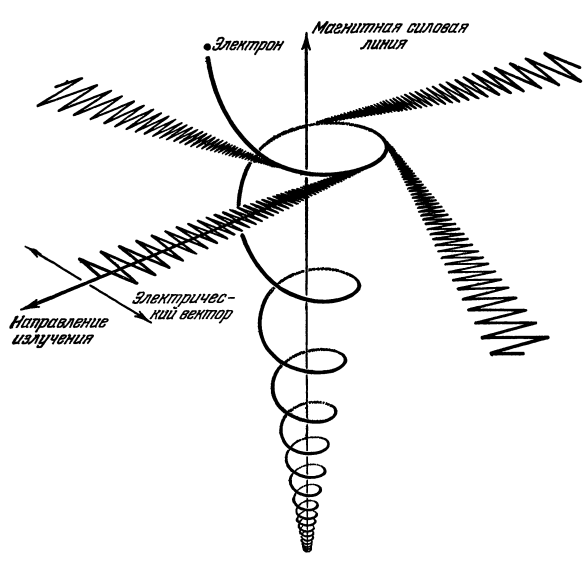
\includegraphics[width=0.3\textwidth]{synchrotron_radiation.png}
	\caption{
		К объяснению синхротронного механизма радиоизлучения.
	}
	\label{fig:synchrotron_radiation}
\end{figure}
\newpage
\subsection{Реликтовое излучение}
Реликтовое микроволновое излучение, пронизывающее весь Космос и несущее информацию о Большом взрыве. В нашу эпоху его спектр соответствует излучению абсолютно черного тела с температурой 2,725 K, так что (в соответствии с формулой Планка) максимум спектральной интенсивности приходится на длину волны 1,9 мм.

\subsection{Излучение плазмы}
Излучение плазменных волн, рожденных в атмосферах звезд и планет (обычно при участии магнитных полей). К примеру, Юпитер помимо теплового радиоизлучения выдает всплески поляризованных радиоволн, генерируемых движением заряженных частиц в верхних слоях атмосферы. Их источником служит и солнечная плазма.


%-------------------------------------------------
\clearpage
\sloppy
\printbibliography
%-------------------------------------------------
\end{document}

